\documentclass[10pt]{beamer}
\setbeamertemplate{navigation symbols}{}%remove navigation symbols
\usepackage{booktabs}
\usepackage{hyperref}
\usepackage{subfig}
\usepackage{tcolorbox}

\usefonttheme{professionalfonts}
%\usefonttheme{serif}

\usepackage{fontspec}
%\usepackage{kantlipsum}
\setbeamerfont{note page}{family*=pplx,size=\footnotesize}
\useoutertheme{infolines}

\usepackage[framemethod=tikz]{mdframed}
\usetikzlibrary{shadows}
\usepackage{pdfpages}
\newmdenv[shadow=true,shadowcolor=black,font=\sffamily,rightmargin=8pt]{shadedbox}
\usepackage{pifont,xcolor}% http://ctan.org/pkg/{pifont,xcolor}
\definecolor{myblue}{RGB}{49,54,149}
\definecolor{myred}{RGB}{165,0,38}
\usepackage{graphicx}
\usepackage{caption}
\newcommand{\lenitem}[2][.55\linewidth]{\parbox[t]{#1}{#2\strut \strut}}

\usetheme{Frankfurt}

   \usefonttheme{professionalfonts} 
\newenvironment{variableblock}[3]{%
  \setbeamercolor{block body}{#2}
  \setbeamercolor{block title}{#3}
  \begin{block}{#1}}{\end{block}}
\usecolortheme{dove}
\usepackage{fancybox}
\setbeamercolor{block title}{bg=white,fg=black}
\newenvironment{fminipage}%
{\begin{Sbox}\begin{minipage}}%
{\end{minipage}\end{Sbox}\fbox{\TheSbox}}

\newcommand{\itemcolor}[1]{% Update list item colour
  \renewcommand{\makelabel}[1]{\color{#1}\hfil ##1}}

\newcounter{tmpc}
%\usefonttheme{structuresmallcapsserif}
\setbeamercolor{section in head/foot}{fg=black, bg=white}

\setbeamertemplate{frametitle}
{
    \nointerlineskip
    \begin{beamercolorbox}[sep=0.3cm,ht=1.8em,wd=\paperwidth]{frametitle}
        \vbox{}\vskip-3ex%
        \strut\insertframetitle\strut
        \vskip-1.2ex%
    \end{beamercolorbox}
}
\addtobeamertemplate{frametitle}{\vskip0.5ex}{}
\makeatletter
\setbeamertemplate{footline}
{
  \leavevmode%
  \hbox{%
  \begin{beamercolorbox}[wd=.875 \paperwidth,ht=2.25ex,dp=1ex,left]{section in head/foot}%
    \usebeamerfont{author in head/foot}\quad \quad \insertshorttitle
 \end{beamercolorbox}%
 \begin{beamercolorbox}[wd=.125\paperwidth,ht=2.25ex,dp=1ex,right]{section in head/foot}%
    \usebeamerfont{date in head/foot} \quad \quad
    \insertframenumber{} / \inserttotalframenumber\hspace*{2ex} 
  \end{beamercolorbox}}%
  \vskip0pt%
}
\let\@@magyar@captionfix\relax
\makeatother

\def\mf{
\begin{itemize}
\item Item
\end{itemize}
}
%\setbeamercolor{itemize item}{fg=yellow,bg=white}
%\setbeamertemplate{itemize items}[circle]
\setbeamercolor{enumerate item}{ fg=red}
\setbeamercolor{item projected}{bg=myblue}

\usepackage{listings}

\lstdefinestyle{BashInputStyle}{
  language=bash,
  basicstyle=\small\sffamily,
  numbers=left,
  numberstyle=\tiny,
  numbersep=5pt,
  framexleftmargin=3mm,
  frame=shadowbox, rulesepcolor=\color{gray},
  numberstyle=\normalfont\tiny\color{myred},
%  fillcolor=\color{gray},
  rulecolor=\color{black},
  columns=fullflexible,
  backgroundcolor=\color{white},
  linewidth=0.9\linewidth,
  xleftmargin=0.1\linewidth
}


\begin{document}

\section{Title/Intro}
\subsection{}
\small
\title{The Architecture of Genome Wide Study\vspace{-.2in}} 
\author{Melinda Mills and \textbf{Charles Rahal}\\ Department of Sociology and Nuffield College \\ University of Oxford \\ \vspace{0.15in} Departmental Seminar, 11th June, 2018}
 \date{}
\frame{\titlepage 
\begin{center}
 \vspace{-0.5in}
 \includegraphics[width=0.45\textwidth]{helix_wordcloud_1250_5000_black.pdf}\\ \vspace{0.2in}
%\color{myblue}Postdoctoral Seminar -- Nuffield College \color{black}\\ \vspace{0.1in}
Replication/Supplementary Material: \color{myblue}\url{https://github.com/crahal}\color{black}\\ 
Comments/Questions/Suggestions: \color{myred}\url{charles.rahal@sociology.ox.ac.uk}\\
 \end{center}
}

\subsection{}
\frame{
\frametitle{General Introduction}
Most speakers in this series present a multitude of papers or summarize their work. \\ \vspace{0.1in} 
My interests are extremely varied in general. Some specific examples:\vspace{0.05in} 
\begin{itemize}
\item Econometric Methods (mostly spatial and time series).
\item Social Mobility and Mortality (applied projects focusing on `elites').
\item Residential Market Policies. (discrimination and affordability for HB recipients)
\item Civic Technology (public procurement and corporate lobbying).
\item ... and of course, Socio-genomics \& the Sociology of Genomics.  \\ \vspace{0.1in}
\end{itemize}
Unifying theme: unstructured data, `big data' or some methodological advancement.\\ \vspace{0.1in}
This involves a lot of open-source development on GitHub (see projects there).\\ \vspace{0.1in}
However, today we'll just focus on one paper: `The Architecture of GWAS'. \\ \vspace{0.1in}
Come to Belfast next week if you want to see a different talk!
}


\subsection{}
\frame{
\frametitle{Introduction to `The Architecture of GWAS'}
\begin{itemize}
\item Joint work with Melinda Mills from my time in her team. \\ \vspace{0.1in}
\item Started out as a `Genomics is WEIRD' style review, but contiunously evolved. \\ \vspace{0.1in}
\item It now represents a toolkit for and analysis of the (social-)architecture of GWAS. \\ \vspace{0.1in}
\item It is a data-driven response to `folk theorems' and qualitative commentaries.\\ \vspace{0.1in}
\item Key idea: link multiple data sources (`cohorts') to understand what drives genetic discovery.
\end{itemize}
\begin{figure}
\centering
\begin{minipage}{.33\textwidth}
  \centering
  \includegraphics[width=.75\linewidth]{gwascatlogo.jpg}
  \label{fig:test1}
\end{minipage}%
\begin{minipage}{.33\textwidth}
  \centering
  \includegraphics[width=.75\linewidth]{pubmedlogo.png}
  \label{fig:test2}
\end{minipage}
\begin{minipage}{.33\textwidth}
  \centering
  \includegraphics[width=.75\linewidth]{EuropePMC1.png}
  \label{fig:test2}
\end{minipage}
\end{figure}
}

\subsection{}
\frame{
\frametitle{But what is a `GWAS'?}
What is a \textbf{G}enome \textbf{W}ide \textbf{A}association \textbf{S}tudy?:\\ \vspace{0.15in}
\begin{figure}
\includegraphics[width=.75\linewidth]{DM_header.png}
%\captionof{figure}{A figure}
\label{fig:test1}
\end{figure}
\begin{itemize}
\item An observational study of a genome-wide set of genetic variants across individuals.\\
\item Focuses on associations between \textbf{S}ingle-\textbf{N}ucleotide \textbf{P}olymorphisms and traits.\\
\item Traits can be related to disease (i.e. neoplasty), body measurements (ie anthropometry) or behaviour (i.e. \textbf{H}uman \textbf{R}eproductive \textbf{B}ehaviour).\\ 
\item EA3: N=\textasciitilde1.1m people to explain 11-13\% of variance of educational attainment.\\
\end{itemize}
}

\subsection{}
\frame{
\frametitle{Data and Methods}
We use the NHGRI-EBI Catalog: a curated database of published SNP-trait associations. \\ \vspace{0.1in}
Every two weeks, new studied updated, periodically adding new fields.\\ \vspace{0.1in}
We link the PUBMEDID field to various PubMed \textbf{A}pplication \textbf{P}rogram \textbf{I}nterfaces. \\ \vspace{0.1in}
All analysis is done in Python 3: specifically an \href{https://github.com/crahal/architectureofGWAS/blob/master/Code/An\%20IPython\%20Notebook\%20For\%20'The\%20Architecture\%20of\%20GWAS'.ipynb}{ \color{myblue}IPython Notebook}. \\ \vspace{0.1in}
Notable Python libraries in use include matplotlib, pandas, Network-X and BioPython. \\ \vspace{0.1in}

We provide a support functions to:
\begin{enumerate}
\setbeamercolor{enumerate subitem}{fg=red!80!black}
\setbeamertemplate{enumerate items}[default]
\item Scrape and clean the various Catalog data.
\item Call and parse various \textbf{A}pplication \textbf{P}rogram \textbf{I}nterfaces.
\item Perform regular expressions based execises to link to the Catalog to API data.\\ \vspace{0.1in}
\end{enumerate}
At the heart is a core data science exercise, where 90\% of the game is wrangling. \\ \vspace{0.1in}
For remainder of this presentation we'll just focus on the outputs rather than methods.

}


\section{An Overview of GWAS}
\subsection{}
\frame{
\frametitle{Some Basic Facts About GWAS}
\begin{itemize}
\item There are currently: 3314 GWAS papers published (first on 2005-03-10).\\ \vspace{0.05in}
\item However, only: 10 papers were published in 2005 and 2006 combined.\\ \vspace{0.05in}
\item This entails 4943 unique Study Accessions across 2909 unique Diseases or Traits.\\ \vspace{0.05in}
\item The total number of Associations found is currently: 67230.\\ \vspace{0.05in}
\item The average number of Associations found per paper is: 13.6.\\ \vspace{0.05in}
\item Mean P-Value for the strongest SNP risk allele is: 1.5748e-06.\\ \vspace{0.05in}
\item The number of associations reaching the 5e-8 threshold is 33026.\\ \vspace{0.05in}
\item The journal to feature the most GWAS since 2005-03-10 is: Nature Genetics.\\ \vspace{0.05in}
\item Total number of journals publishing GWAS is 436.\\ \vspace{0.05in}
\item The study with the largest number of authors has: 559 authors.\\ \vspace{0.05in}
\end{itemize}
}

\subsection{}
\frame{
\frametitle{Growth of GWAS}
\begin{center}
\begin{figure}
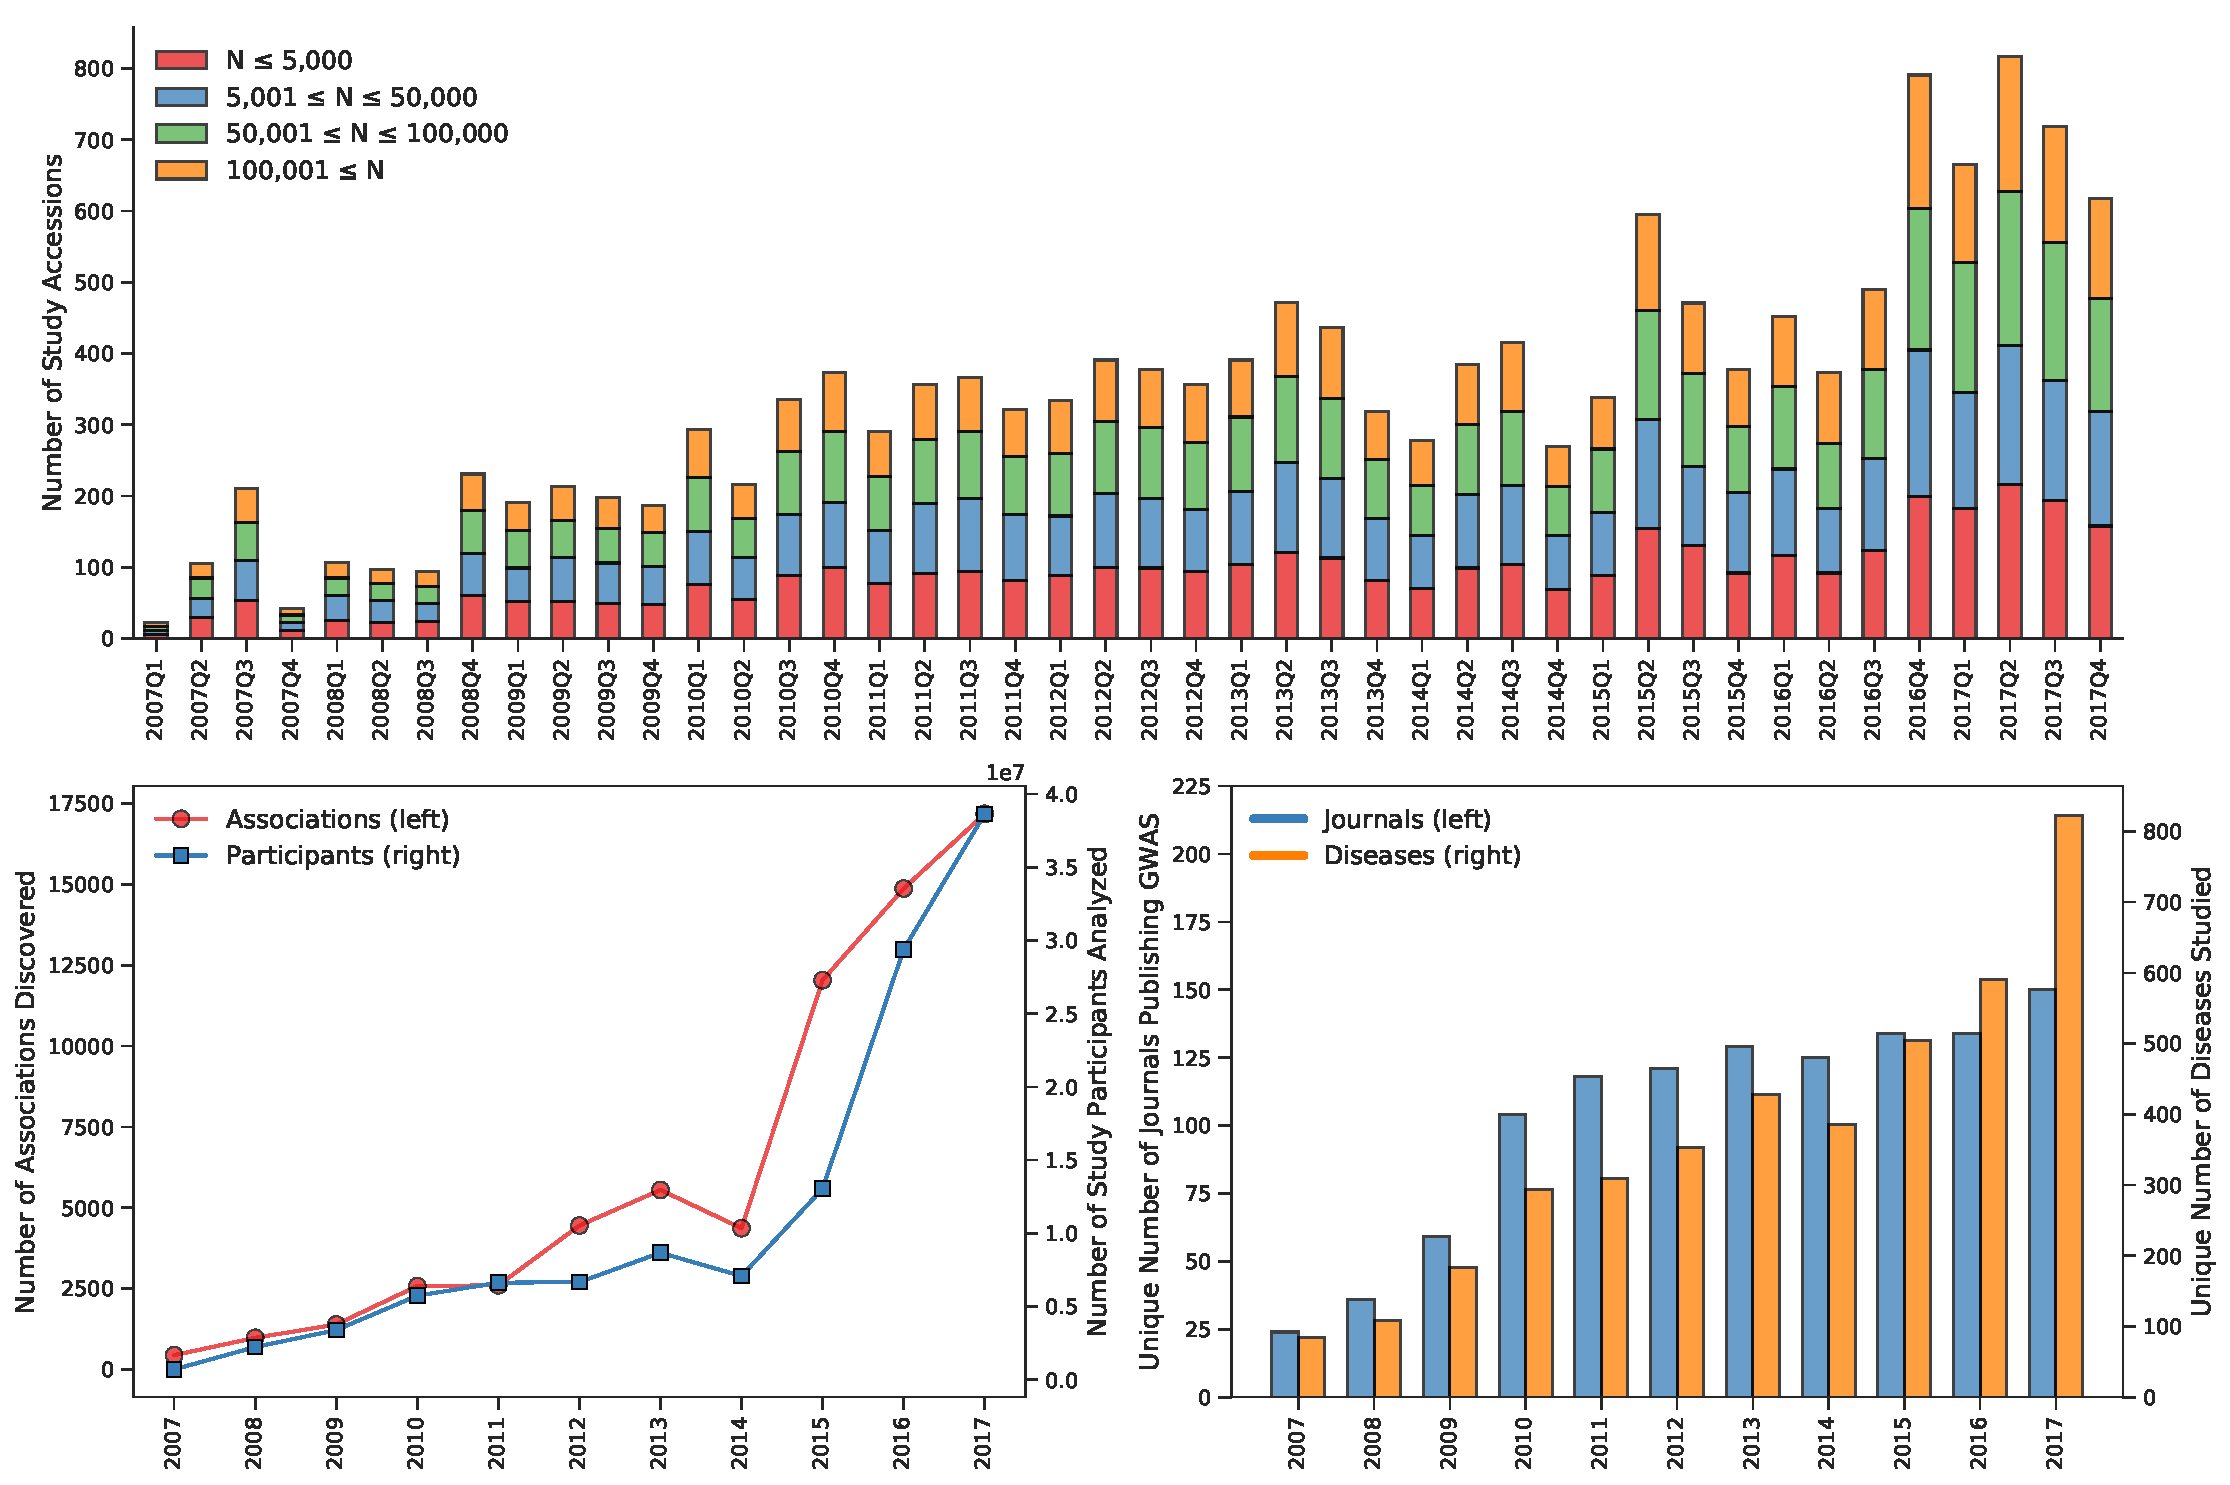
\includegraphics[width=0.75\textwidth, angle=0]{GWAS_Popularity.pdf}
\end{figure}
\end{center}
}

\section{Participants}
\subsection{}
\frame{
\frametitle{Participant Ancestry}
\begin{center}
\begin{figure}
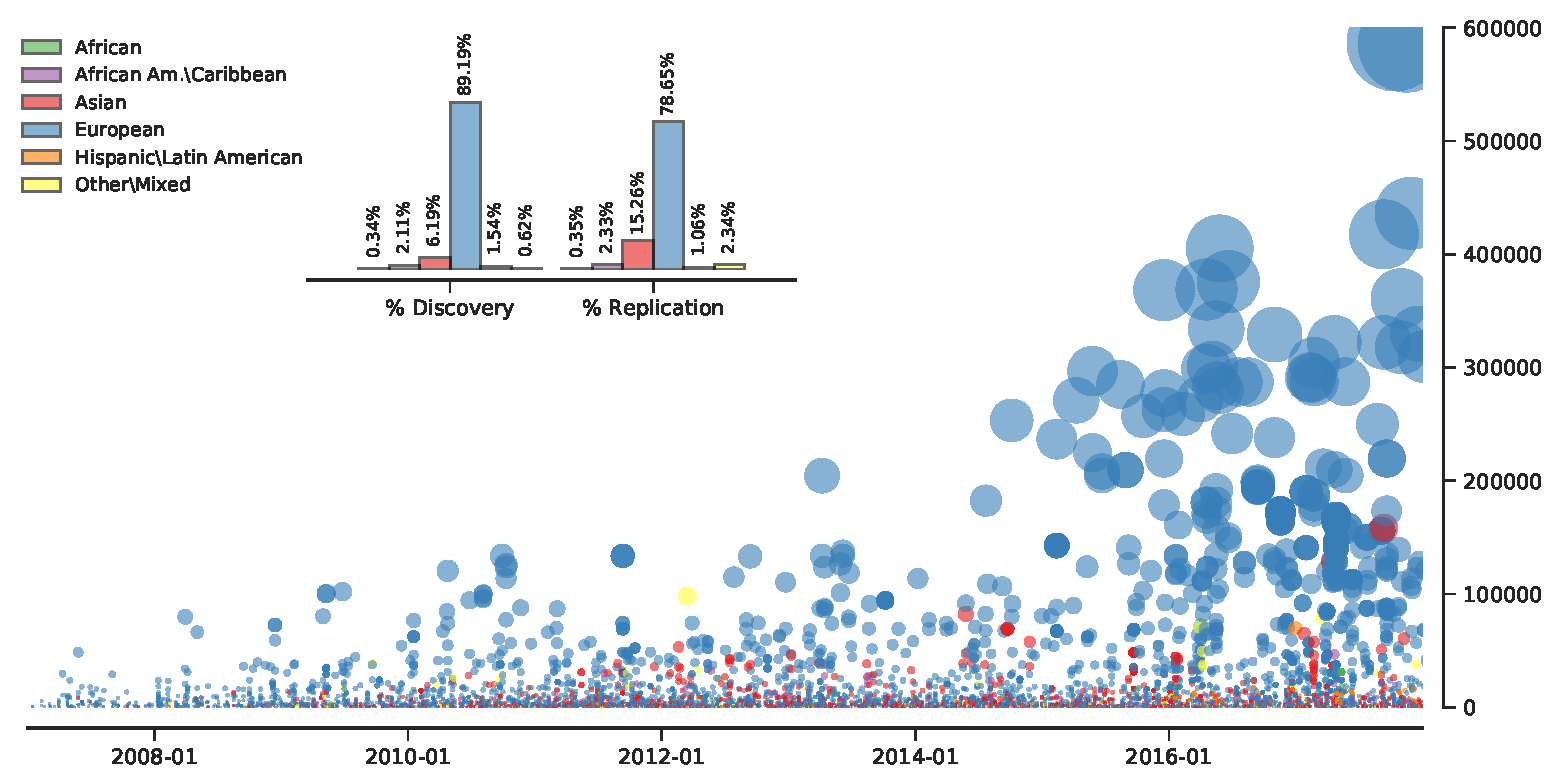
\includegraphics[width=0.75\textwidth, angle=0]{Ancestral_Plots.pdf}
\end{figure}
\end{center}
\begin{itemize}
\item Critical public health debate about `personalized medicine': personalised for who?\\ \vspace{0.05in}
\item Larger genetic variation in non-Europeans aids discovery. Simple arithmetics shows three (four) times more discoveries per person for African (Hispanics) ancestry.
\end{itemize}
}

\subsection{}
\frame{
\frametitle{Participant Ancestry Over Time}
\begin{table}[]
\centering
\scalebox{0.85}{
\begin{tabular}{rcccccc} \toprule
     & Eur & Asian & African & H/L Am. & Other/Mixed &  AA/AC \\ \midrule
2007 & 95.47 & 2.14  & 0.01 & 0.72 & 1.18 & 0.49\\
2008 & 95.10 & 3.06  & 0.00 & 0.00 & 1.27 & 0.57\\
2009 & 88.17 & 7.10  & 0.26 & 0.22 & 3.36 & 0.88\\
2010 & 86.54 & 10.13 & 0.27 & 0.06 & 2.49 & 0.50\\
2011 & 78.19 & 15.88 & 0.15 & 0.40 & 1.72 & 3.66\\
2012 & 71.15 & 20.04 & 0.32 & 0.91 & 2.96 & 4.62\\
2013 & 81.55 & 12.10 & 0.41 & 0.82 & 0.64 & 4.48\\
2014 & 76.42 & 18.74 & 0.24 & 1.17 & 0.99 & 2.43\\
2015 & 84.47 & 11.89 & 0.37 & 0.96 & 0.66 & 1.66\\
2016 & 90.97 & 4.54  & 0.20 & 1.54 & 1.30 & 1.45\\
2017 & 88.14 & 6.29  & 0.56 & 2.30 & 0.52 & 2.19\\ \bottomrule
\end{tabular}}\\
\tiny{Abreviations: AA/AC: African American or Afro-Caribean, H/L Am: Hispanic or Latin American, Eur: European.}
\end{table}
\begin{itemize}
\item Despite a reduced focus on Europeans c.2011-2014, the upward trend is due to the rise of large national biobanks (U.K. Biobank), biopharmaceutical companies (DeCODE) and personal genetics (23andMe).
\end{itemize}
}


\subsection{}
\frame{
\frametitle{Polyvocality and Scientific Authority}

\begin{itemize}
\item Former analysis is based on a mapping between 182 combinations of `broader ancestries'  identified in the Catalog and our six pre-defined categories.\\ \vspace{0.1in}
\item The Catalog also provides a `free text' field describing the ancestry. \\ \vspace{0.1in}
\item We decompose this to examine `polyvocality' (Panofsky and Bliss, 2017, ASR). \\ \vspace{0.1in}
\item Lets take an example: 
\begin{enumerate}
\setbeamercolor{enumerate subitem}{fg=red!80!black}
\setbeamertemplate{enumerate items}[default]
\item Free text: “19,546 British ancestry individuals from 6,863 families”. \\
\item REs can separate: “19,546” and “British” into two fields for further analysis. \\ \vspace{0.1in}
\end{enumerate}
\item We can isolate 207 and 147 unique terms for discovery and replication respectively. \\ \vspace{0.1in}
\item These are terms for classifying participants in terms of race, region, county, ethnicity or ancestry. \\ \vspace{0.1in}
\item Whether some of these terms are used in ‘logically ambiguous ways’ to propogate authority is for somebody else to decide.
\end{itemize}
}


\subsection{}
\frame{
\frametitle{Country of Recruitment}
\begin{center}
\begin{figure}
\includegraphics[width=0.95\textwidth, angle=0]{Country_Rec_N.pdf}
\end{figure}
\end{center}
}


\subsection{}
\frame{
\frametitle{Continent of Recruitment}
\begin{table}[]
\centering
\scalebox{0.85}{
\begin{tabular}{rcccc} \toprule
Continent & N & \# Studies & N (\%) & \# Studies (\%)\\ \midrule
Africa & 39,742 & 43 & 0.11 & 0.80\\
Asia & 5,180,891 & 1,298 & 14.22 & 24.11\\
Europe & 21,529,123 & 1,528 & 59.11 & 28.38 \\
North America & 9,345,005 & 2,380 & 25.66 & 44.21\\
Oceania & 302,888 & 107 & 0.83 & 1.99 \\
Seven seas & 1,389 & 1 & 0.00 & 0.02 \\
South America & 22,256 & 27 & 0.06 & 0.50\\ \bottomrule
\end{tabular}}
\end{table}
\begin{itemize}
\vspace{0.1in}
\item Only 0.11\% of participants are recruited from Africa, 0.06\% from South America. \\ \vspace{0.05in}
\item 84.77\% of participants come from either North America or Europe.\\ \vspace{0.05in}
\item But... approximately 76.2\% of the current global population reside in Asia or Africa!\\ \vspace{0.05in}
\end{itemize}
}


\subsection{}
\frame{
\frametitle{Cohort Resampling}
\begin{table}[]
\centering
\scalebox{0.85}{
\begin{tabular}{rccccc} \toprule
Cohort & Count & N       & Recruitment     & Age Range \\ \midrule
Rotterdam Study & 373   & 14,926  & Netherlands     & 55-106\\
ARIC & 187   & 15,792  & US & 45-64 \\
Framingham & 183   & 15,447  & US & 5-85*\\
CHS & 163 & 5,888   & US & 65+  \\
1958BC & 144 & 17,634 & UK & 0+ \\
SHIP & 120 & 4,308 & Germany & 20-79 \\
TWINSUK & 120   & 12,000  & UK, Ireland & 18-103 \\
Nurses Health Study & 112   & 121,700 & US & 30-55 \\
AGES & 110   & 30,795  & Iceland & 33-84 \\
EPIC & 108   & 521,330 & 10 EU countries & 21-83**\\ \bottomrule
\end{tabular}}\\
\footnotesize{*denotes originally 30-62 years, ** denotes variation by country.}
\end{table}
\normalsize
\begin{itemize}
\item Ten most frequently utilized cohorts: largest 1,000 GWAS (01/09/2017). \\
\item This was the result of an \textbf{extensive} manual data collection exercise.\\ 
\item Analyzes resampled demographics of cohorts which are repeatedly analyzed. \\
\item Many thanks to Pilar, Domant\`{e} and Xuejie for all their help with this work!
\end{itemize}
}



\section{Funders}
\subsection{}
\frame{
\frametitle{Which Countries Fund GWAS?}
\begin{table}[]
\centering
\scalebox{0.85}{
\begin{tabular}{rcc} \toprule
 & \# Studies & Percent (\%) \\ \midrule
United States & 39273 & 86.32 \\ 
United Kingdom & 6006 & 13.20 \\
Canada & 165 & 0.36 \\
International & 38 & 0.08\\
Austria & 6 & 0.01\\
None & 6 & 0.01\\
Italy & 5 & 0.01 \\ \bottomrule
\end{tabular}
}
\end{table}
\begin{itemize}
\item There are 87 unique funders returned from PubMed Central.
\item There are 12167 unique grants returned from PubMed Central.
\item Each study has an average of 13.73 grants funding it.
\item The most frequently acknowledged grant is GrantID P30 DK063491 (182 times).
\end{itemize}

}


\subsection{}
\frame{
\frametitle{Which institutions fund GWAS?}
\begin{table}[]
\centering
\scalebox{0.85}{
\begin{tabular}{rccc} \toprule
 & Grant Contributions & GrantCountry & \% of Total \\ \midrule
NHLBI NIH HHS & 12388 & United States & 27.23 \\
NCI NIH HHS & 5013 & United States & 11.02 \\
NIA NIH HHS & 3872 & United States & 8.51 \\
MRC & 2913 & United Kingdom & 6.4 \\
NIMH NIH HHS & 2593 & United States & 5.7 \\
NIDDK NIH HHS & 2470 & United States & 5.43 \\
NHGRI NIH HHS & 1718 & United States & 3.78 \\
Wellcome Trust & 1608 & United Kingdom & 3.53 \\
NCRR NIH HHS & 1527 & United States & 3.36 \\
PHS HHS & 1137 & United States & 2.5 \\ \bottomrule
\end{tabular}}
\end{table}
}

\subsection{}
\frame{
\frametitle{What do they fund?}
\begin{center}
\begin{figure}
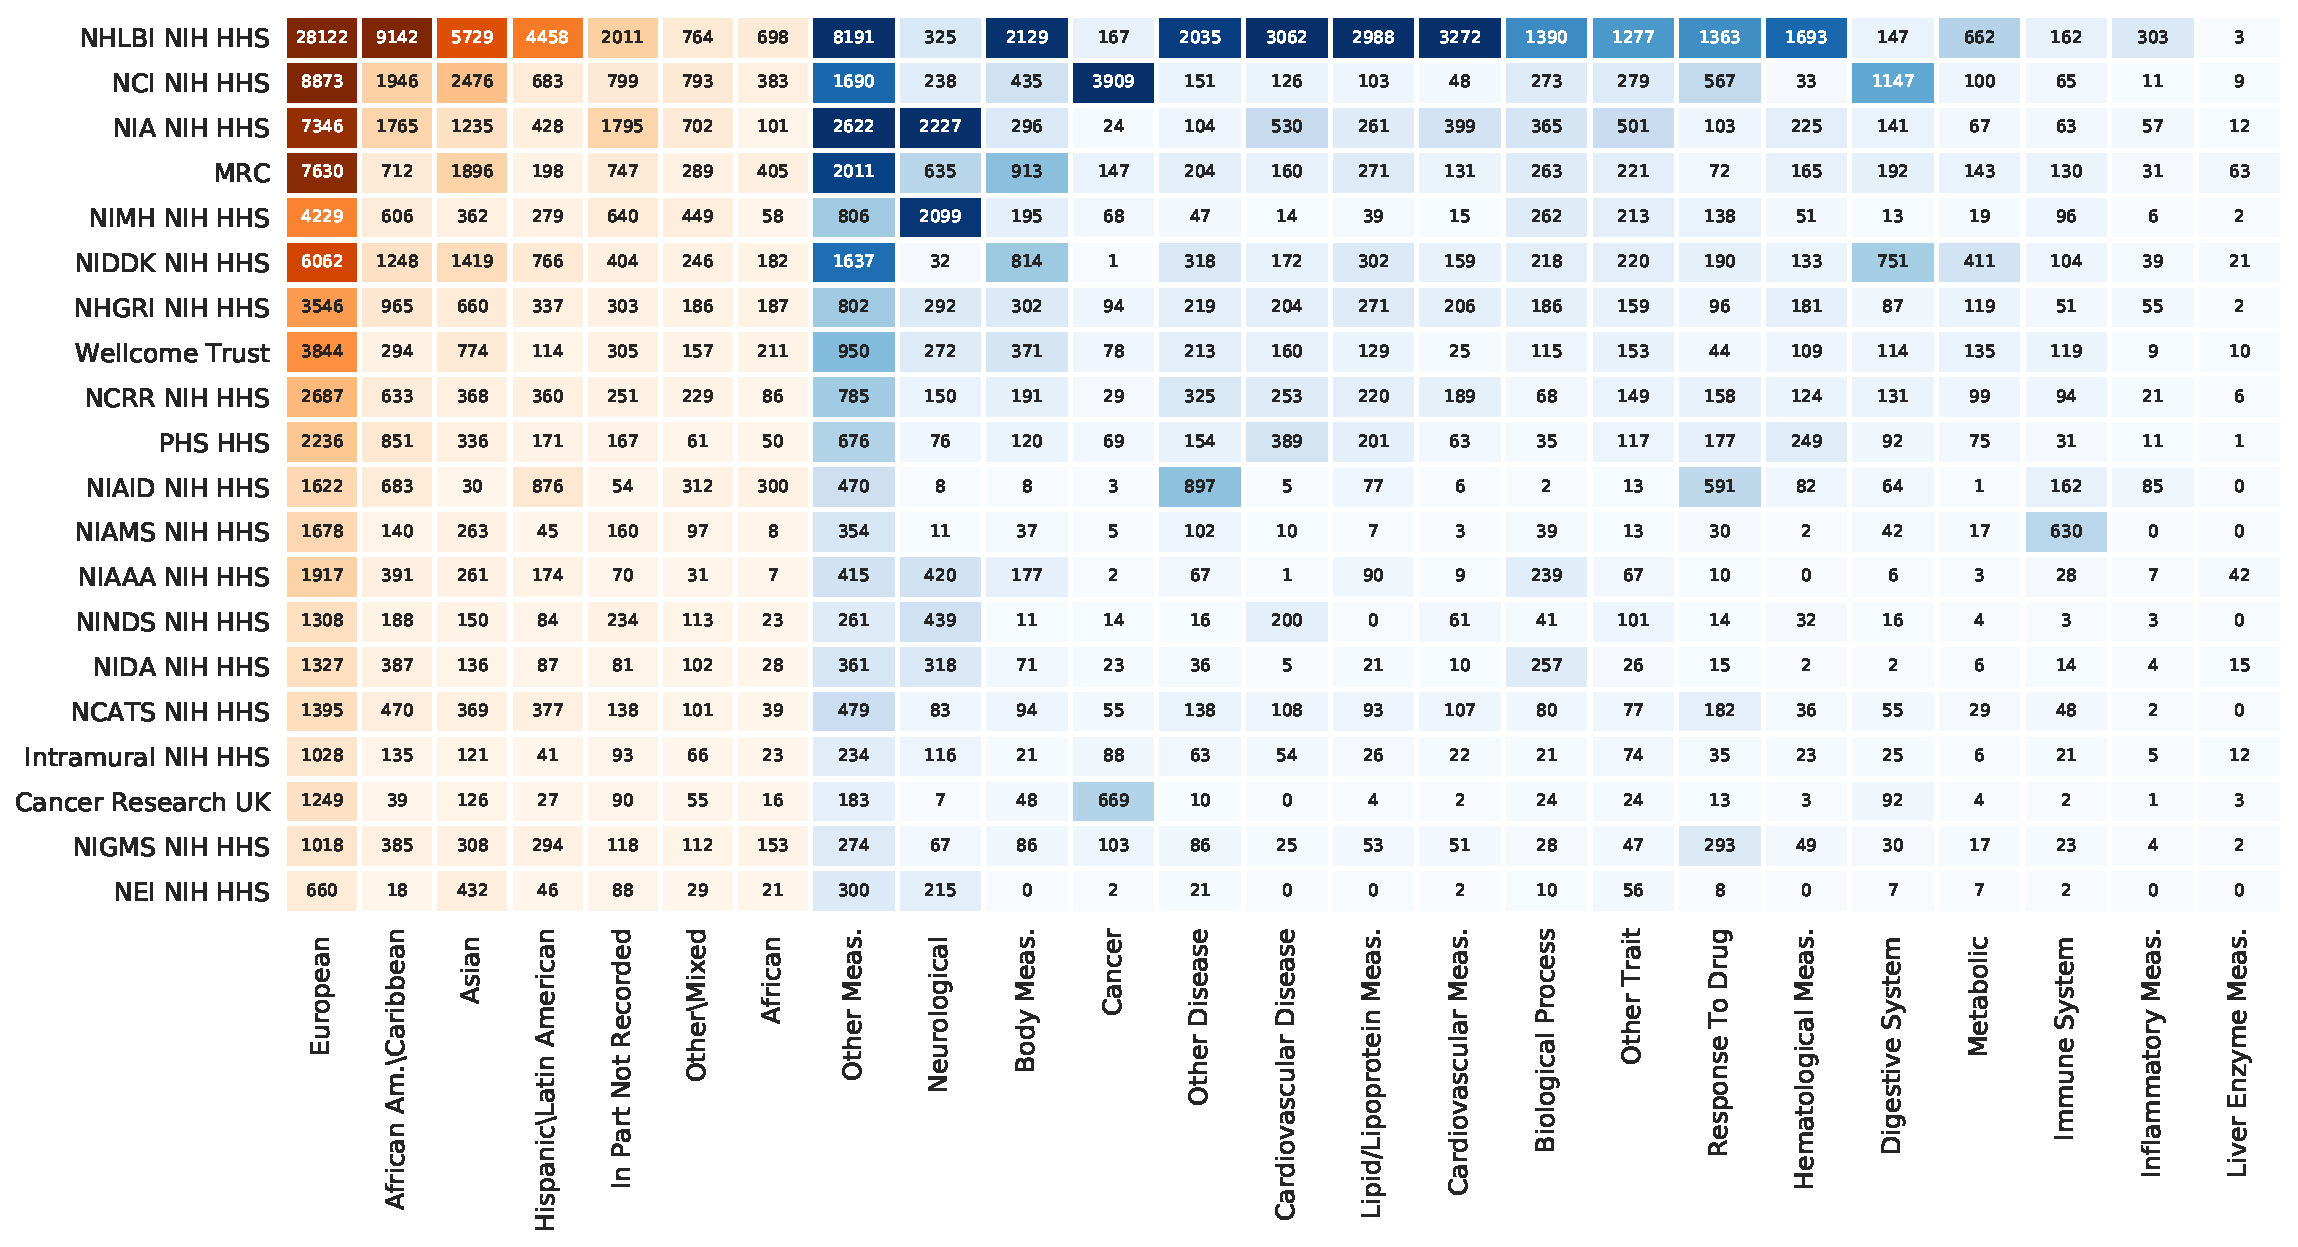
\includegraphics[width=0.925\textwidth, angle=0]{Funder_Heatmap.pdf}
\end{figure}
\end{center}
}

\section{Researchers}
\subsection{}
\frame{
\frametitle{Who are the Most Prolific and Central Authors?}
\begin{table}[]
\centering
\scalebox{0.7}{
\label{my-label}
\begin{tabular}{rccccccc}\toprule
Author & Papers & Cites & GWAS-H & Between & Degree & Country     & Institution           \\ \midrule
K. Stefansson        & 165    & 24434        & 81     & 0.022       & 0.311  & Iceland     & deCode \\
U. Thorsteinsdottir & 132    & 21063        & 74     & 0.007       & 0.246  & Iceland     & deCode  \\
A. G. Uitterlinden   & 257    & 19893        & 72     & 0.017       & 0.353  & Netherlands & Erasmus MC            \\
A. Hofman          & 255    & 21988        & 72     & 0.014       & 0.342  & U.S.        & Harvard \\
C. M van Duijn   & 175    & 17795        & 67     & 0.008       & 0.284  & Netherlands & UMC Rotterdam         \\
C. Gieger       & 155    & 19353        & 66     & 0.012       & 0.274  & Germany     & Helmholtz-Muenchen    \\
H-E. Wichmann       & 109    & 18395        & 66     & 0.009       & 0.233  & Germany     & Helmholtz-Muenchen    \\
G. Thorleifsson    & 112    & 18084        & 66     & 0.007       & 0.235  & Iceland     & deCode   \\
P. Deloukas         & 96     & 16812        & 62     & 0.007       & 0.229  & U.K.        & Queen Mary UoL        \\
F. Rivadeneira   & 184    & 15537        & 62     & 0.008       & 0.277  & Netherlands & UMC Rotterdam  \\ \bottomrule
\end{tabular}}
\end{table}
\begin{itemize}
\item GWAS H-Index: published $h$ papers each of which has at least $h$ citations, but only for papers in the Catalog (cites can be from anywhere). \\ \vspace{0.025in}
\item All these authors are either proprietors of large datasets or cohort leaders. \\ \vspace{0.025in}
\item These metrics are highly correlated in general ($\rho$>=0.5).\\ \vspace{0.025in}
\item Slightly further down the list are some close friends of the department, such as: Augustine Kong (28th), Cecilia Lindgren (144) and John Perry (150).
\end{itemize}
}


\subsection{}
\frame{
\frametitle{Structural Gender Bias in Authorship Position}
\begin{itemize}
\item Only two of ten authors in the table are female, leading us to consider gender bias.\\ \vspace{0.05in}
\item A number of excellent studies discuss gender imbalance in science.\\ \vspace{0.05in}
\item We use a carefully prepared international name dictionary with 40,000 entries.\\ \vspace{0.05in}
\item Men  contribute 63.05\% of GWAS authorships: representing 59.53\% unique authors.\\ \vspace{0.05in}
\item Compare to recent estimates that 27.27\% of academic authorships between 1990-2011 are on aggregate female,\\ \vspace{0.05in}
\begin {itemize}
\item This increases to 29.3\% filtering for Molecularand  Cell Biology.\\ \vspace{0.05in}
\item And to 32.4\% for the specific subdiscipline of Human Genomics.\\ \vspace{0.05in}
\end{itemize}
\item Most importantly we show substantial variation across authorship position: \\ \vspace{0.05in}
\begin{itemize}
\item 43.30\% authors in the ‘first author’ or junior are female. \\ \vspace{0.05in}
\item This decreases to just 29.27\% for authorships in the senior ‘last author’ position. \\ \vspace{0.05in}
\end{itemize}
\end{itemize}
}

\subsection{}
\frame{
\frametitle{Gendered Study of Traits}
\begin{center}
\begin{figure}
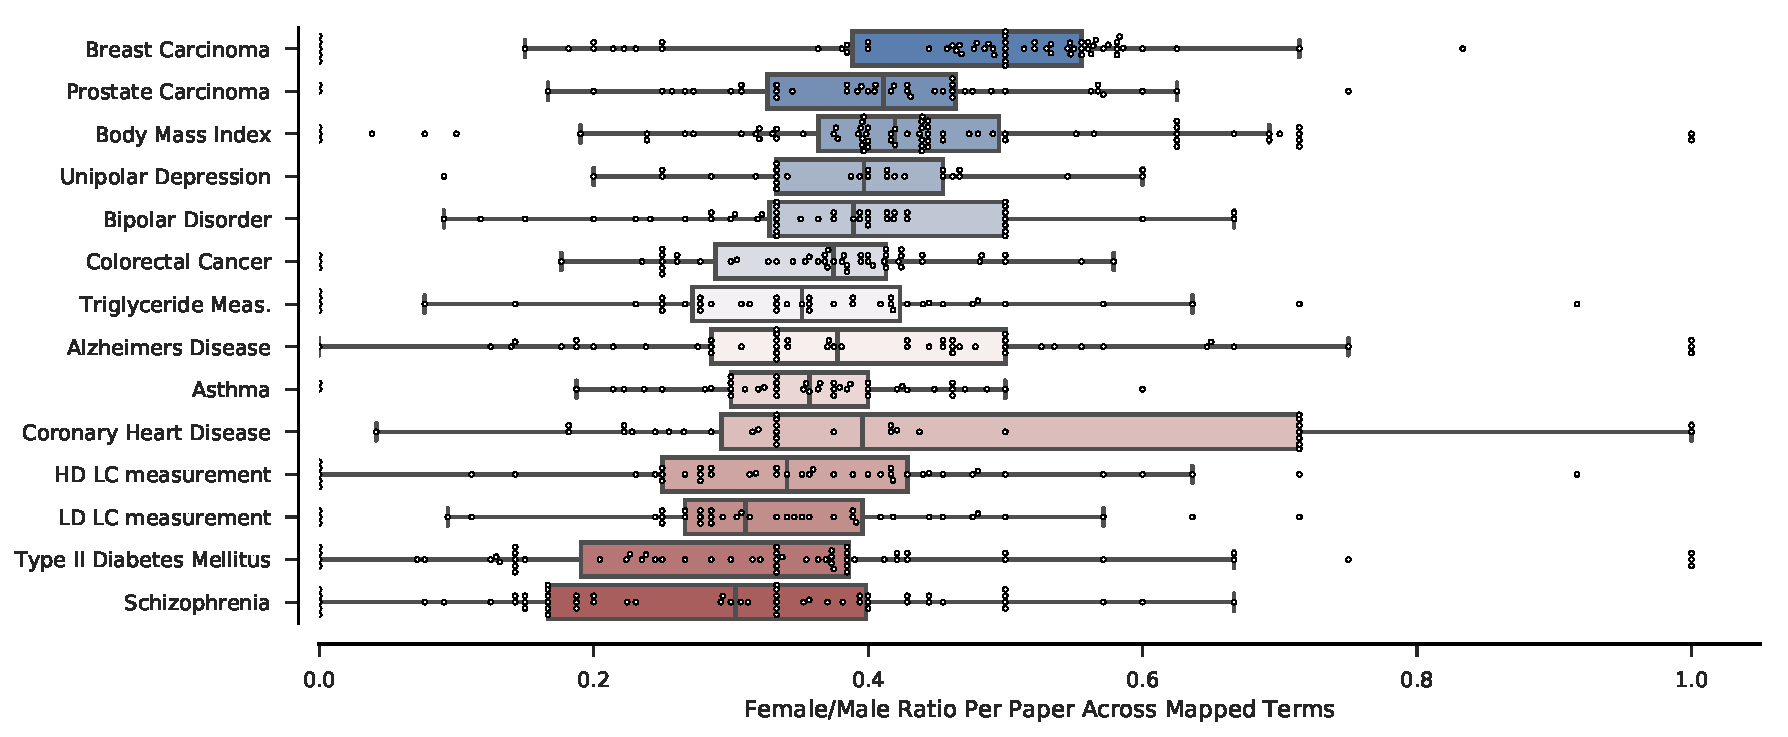
\includegraphics[width=0.925\textwidth, angle=0]{Gender_by_Subjects.pdf}
\end{figure}
\end{center}
\begin{itemize}
\item Concentration of female authorship in studies of Breast Carcinoma (50.5\%). \\ \vspace{0.05in}
\item Male authors are concentrated on Schizophrenia and Type II Diabetes \\ \vspace{0.1in}
\end{itemize}
}

\subsection{}
\frame{
\frametitle{Contributing Collectives (Consortium)}
We also analyze collectives (`consortiums') associated with various PubMed IDs.\vspace{0.05in}
Dictionary based replacement: eg. ‘AGEN’ and ‘AGEN Consortium’ map to same entity.\vspace{0.05in}
\begin{itemize}
\item We see a total of 612 different collectives.\vspace{0.05in}
\item A total of 753 papers are contributed to by at least one collective.\vspace{0.05in}
\item A total of 1429 collective contributions are made. \\ \vspace{0.1in}
\end{itemize}
The most frequently seen Consortium are:
\begin{enumerate}
\setbeamercolor{enumerate subitem}{fg=red!80!black}
\setbeamertemplate{enumerate items}[default]
\item Wellcome Trust Case Control Consortium (42)
\item CHARGE (38)
\item Wellcome Trust Case Control Consortium 2 (32)
\item DIAGRAM (28)
\item LifeLines Cohort Study (28)
\end{enumerate}
}

\section{Conclusion}
\subsection{}
\frame{
\frametitle{Conclusion}
\begin{itemize}
\item Existing reviews are mostly narrative or extremely narrow commentaries. \\ \vspace{0.1in}
\item Our genetic knowledge base is limited to UK, US and Icelandic particpants. \\ \vspace{0.1in}
\item There exist structural clusterings of power in authorship and divides of gender. \\ \vspace{0.1in}
\item We provide the tools to analyze genomics as it enters the exome sequencing era. \\ \vspace{0.1in}
\item Predict that UK Biobank (94\% `white') and 23andMe (77\% European) will decrease diversity. \\ \vspace{0.1in}
\item Multiple science of science policy type recommendations, but two scientometric:
\begin{enumerate}
\setbeamercolor{enumerate subitem}{fg=red!80!black}
\setbeamertemplate{enumerate items}[default]
\item Mandate ORCID registration and a standard return from bibliometric APIs.\\ \vspace{0.025in}
\item Register each cohort with a unique DOI.\\ \vspace{0.025in}
\end{enumerate}
\end{itemize}
\vspace{0.2in}
}	






\frame{
\frametitle{}
\begin{center}
\begin{figure}
\includegraphics[width=0.825\textwidth, angle=0]{cartoon.png}
\end{figure}
\end{center}
\vspace{0.15in}
\fbox{\begin{minipage}{37.5em}
Thanks again to Pilar, Domant\`{e} and Xuejie, and of course Melinda. Useful comments recieved from Felix Tropf, the Sociogenome reading group and friend of the Department Ben Domingue. None of this possible without their help in one way or another.
\end{minipage}}
}


\end{document}
